\documentclass[12pt,twosides]{article}
\usepackage{jmlda, amssymb, amsmath}
\usepackage{hyperref}
\usepackage{graphicx}
%\NOREVIEWERNOTES

\graphicspath{{../pics/}}
%\epstopdfDeclareGraphicsRule{.pdf}{png}{.png}{convert #1 \OutputFile}
%\DeclareGraphicsExtensions{.png,.pdf}

\title
[Качество структуры белка с  графовыми сетями]
{Оценка качества прогнозирования структуры белка с использованием графовых нейронных сетей.}
\author
[Северилов~П.А.] 
{Северилов~П.А.$^1$} 
% [] список авторов, выводимый в заголовок; не нужен, если он не отличается от основного
\thanks
	{Научный руководитель:  В.В. Стрижов
		}
\email
{severilov.pa@phystech.edu}
\organization
{$^1$Московский физико-технический институт (МФТИ)}
\abstract
{Оценка качества предсказания белковой структуры является важной и пока открытой проблемой в структурной биоинформатике (биологии). В работе проводится анализ графовых нейронных сетей в комбинации со сверточными применительно к данной задаче.
	
\bigskip
\textbf{Ключевые слова}: \emph {белок, графы, графовые нейронные сети, GCN}.}


\begin{document}
	\maketitle
	%\linenumbers
	
	\section{Введение}
	
	Понимание белковых структур и выполняемых задач помогают контроллировать биологические процессы. Белки спонтанным образом принимают форму в различных средах [?] — форма диктует функционал. Но из имеющихся последовательностей аминокислот в белке трудно определить, в какую форму произойдет сворачивание. Идентификация структуры занимает большое количество времени и ресурсов, к тому же, не всегда возможна. 
	
	Вычислительные методы, которые решают задачу предсказания структуры в основном состоят из двух этапов[?]: генерация конформаций белка из их аминокислотных последовательностей и оценивание качества предсказания. В данной работе рассматривается только вторая задача. Данная проблема является крайне важной[?]. Каждые два года проводятся соревнования Critical Assessment of protein Structure Prediction (\href{http://predictioncenter.org/}{CASP}) по решению этой задачи.
	
	До недавнего времени лучшими методами предсказания стурктуры считались[?...?] объединение подходов, основанных на функциях, предназначенных для узкого класса белков. Методы глубинного обучения превзошли \cite{AlphaFold} эти результаты.
	
	Основные результаты в этой области полагаются на сверточные нейронные сети (CNN) \cite{10.1093/bioinformatics/btz122}. Т.к. имеющиеся данные представляют собой трехмерные координаты атомов, то предлагается использовать графовые архитектуры нейронных сетей в комбинации с уже имеющимися архитектурами.
	
	
	\section{Связанные работы}
	To be done \\
	One of the interesting \href{https://github.com/jdlc105/Must-read-papers-and-continuous-tracking-on-Graph-Neural-Network-GNN-progress}{links}
	
	
	\section{Постановка задачи}
		
		\subsection{Задача регрессии}
		Пусть $\mathfrak{D} = (\mathbf{X}, \mathbf{y})$ ~--- заданная выборка, где $\mathbf{X}\in \mathbb{R}^{m\times n\times 3}$ ~--- тензор объект-признак, объекты $\mathbf{x}_i\in \mathbb{R}^{1\times n\times 3}, i=\overline{1,m}$ ~--- это молекулы, каждая из которых описана множеством 3-мерных координат всех ее атомов, а $\mathbf{y} = [y_1,\dots, y_m]^{\mathsf{T}}\in \mathbb{R}^{m\times 1}$ ~--- оценка близости предсказанной и реальной структуры белка. Оценка близости может быть измерена различными метриками: CAD-score\cite{Olechnovic2013CADscoreAN}, LDDT, GDT. В данной работе выбран CAD-score. 
		
		Рассмотривается множество параметрических моделей $\mathfrak{F}$, взятых из класса графовых сверточных нейронных сетей: $\mathfrak{F} = \{\mathbf{f}_k\colon(\mathbf{w}, \mathbf{X})\to  \mathbf{\hat{y}}\mid k \in \mathfrak{K}\}$, где $\mathbf{w} \in \mathbb{W}$ ~-- параметры модели, а $\hat{\mathbf{y}}\in \mathbb{R}^{m\times 1}$ - вектор оценок предсказаний (CAD-scores). 
		
		Рассматривается задача регрессии для предсказания численного значения CAD-score $y_i$ белка на основе его смоделированной пространственной структуры $\mathbf{x}_i$.
		
		Параметры модели $\mathbf{w}\in \mathbb{W}$ подбираются в соответствии с минимизацией функции ошибки на обучении. Определим функцию ошибки
		$\mathfrak{L}(\mathbf{y}, \mathbf{X}, \mathbf{w}) =\left( \mathbf{\hat{y}} - \mathbf{y} \right)^{2}$, где $\mathbf{\hat{y}} = \mathbf{f} (\mathbf{X},\mathbf{w})$ -- CAD-score, предсказанный моделью $\mathbf{f}$, $\mathbf{y}$ -- данный в выборке CAD-score.
		
		\subsection{CAD score}
		Обозначим через $G$ множество всех пар элементов последовательности аминокислот (остатков)  $(i, j)$, имеющих ненулевую площадь контакта $T_{(i, j)}$ в реальной структуре. Затем для каждой пары остатков $(i, j)\in G$ вычисляется площадь контакта $M_{(i, j)}$ смоделированной структуры. 
		Для каждой пары остатков $(i, j) \in G$ определяется разность площадей контакта как абсолютная разница площадей контакта между остатками $i$ и $j$ в реальной $T$ и смоделированной структуре $M$:
		$$\mathrm{CAD}_{(i, j)}=\left|T_{(i, j)}-M_{(i, j)}\right|$$
		
		Для вычислительной стабильности берется ограниченный CAD: $\mathrm{CAD}_{(i, j)}^{\text {bounded}}=\min \left(\mathrm{CAD}_{(i, j)}, T_{(i, j)}\right)$. Таким образом:
		CAD-score для всей структуры определяется как
		$$\mathrm{CAD}_\text{score}=1-\cfrac{\sum_{(i, j) \in G} \mathrm{CAD}_{(i, j)}^{\text {bounded }}}{\sum_{(i, j) \in G} T_{(i, j)}}$$
	
	\section{Теоретическая часть}
	
		\subsection{Представление белков в виде графов}
	  Элементы аминокислотной последовательности рассматриваются как отдельные узлы, чьи связи (ребра) описывают пространственные отношения между ними. 
	
	В общем случае граф $\mathbf{G}$ определяется набором $\mathbf{(V, A)}$, где $\mathbf{V}\in \mathbb{R}^{n \times c}$ определяет вершины или узлы графа, $n$ – число узлов и $c$ – число признаков в каждом узле. Матрица смежности $\mathbf{A}\in \mathbb{R}^{n \times n}$ определяет соединения между $n$ узлами (ребра), где $\mathbf{A}_{ij}$ – сила связи между узлами $i$ и $j$. Используя это определение графа, белковые структуры можно определить как графы, признаки элементов аминокислотной последовательности которых закодированы в элементах $\mathbf{V}$ узлов, а пространственная близость между элементами закодирована в матрице смежности $\mathbf{A}$.
	
		\subsection{Слой свертки графа}
	Дан граф $\mathbf{A}$ и матрица с информацией об узлах $\mathbf{X} \in \mathbb{R}^{n \times c}$.  Слой свертки графа представлен в следующей форме:
	
	$$\mathbf{Z}=f\left(\tilde{\mathbf{D}}^{-1} \mathbf{A} \mathbf{X} \mathbf{W}\right),$$
	
	где $\mathbf{A}$ – матрица смежности графа с добавлением петель, $\tilde{\mathbf{D}}$ это его диагональная матрица степеней вершин, где $\tilde{\mathbf{D}}_{i i}=\sum_{j} \mathbf{A}_{i j}, \mathbf{W} \in \mathbb{R}^{c \times c^{\prime}}$ – матрица параметров свертки обучаемого графа, $f$ – нелинейная функция активации, а $\mathbf{Z} \in \mathbb{R}^{n \times c^{\prime}}$ – выходная матрица.
	
		
	\section{Вычислительный эксперимент}
		
			\subsection{Данные}
			Берутся с соревнований CASP. Для реальной структуры белка берется еще смоделированная структура. Для них вычисляется CAD-score. Модель на тесте предсказывает CAD-score для смоделированной структуры, не имея возможности напрямую вычислить CAD-score по реальной структуре.
			
			Пример анализа одного из белков:
			\begin{figure}[!h]
				\centering
				\begin{minipage}[b]{0.45\textwidth}
					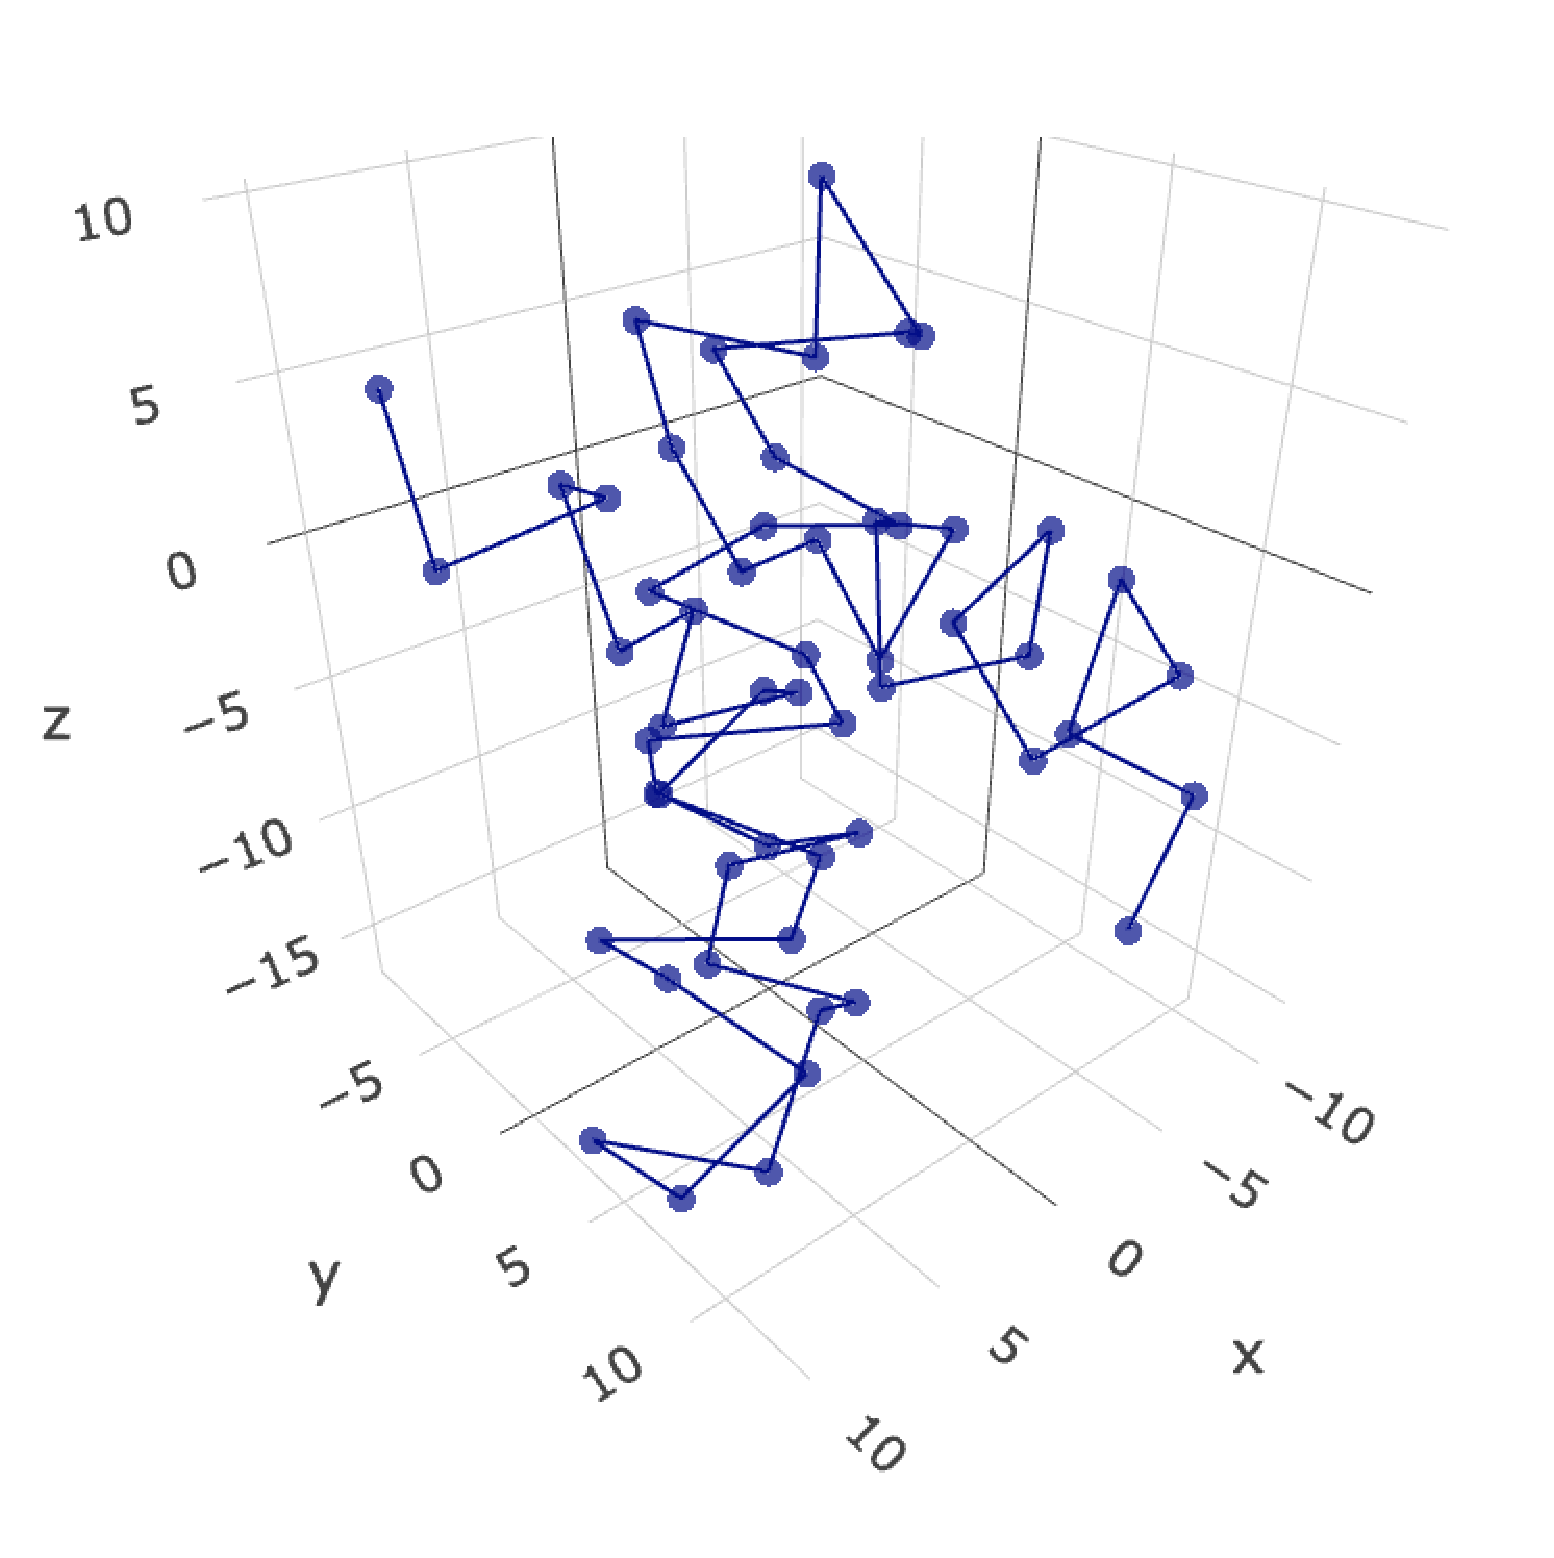
\includegraphics[width=\textwidth]{fig1.pdf}
					\caption{3D структура белка}
				\end{minipage}
				\hfill
				\begin{minipage}[b]{0.45\textwidth}
					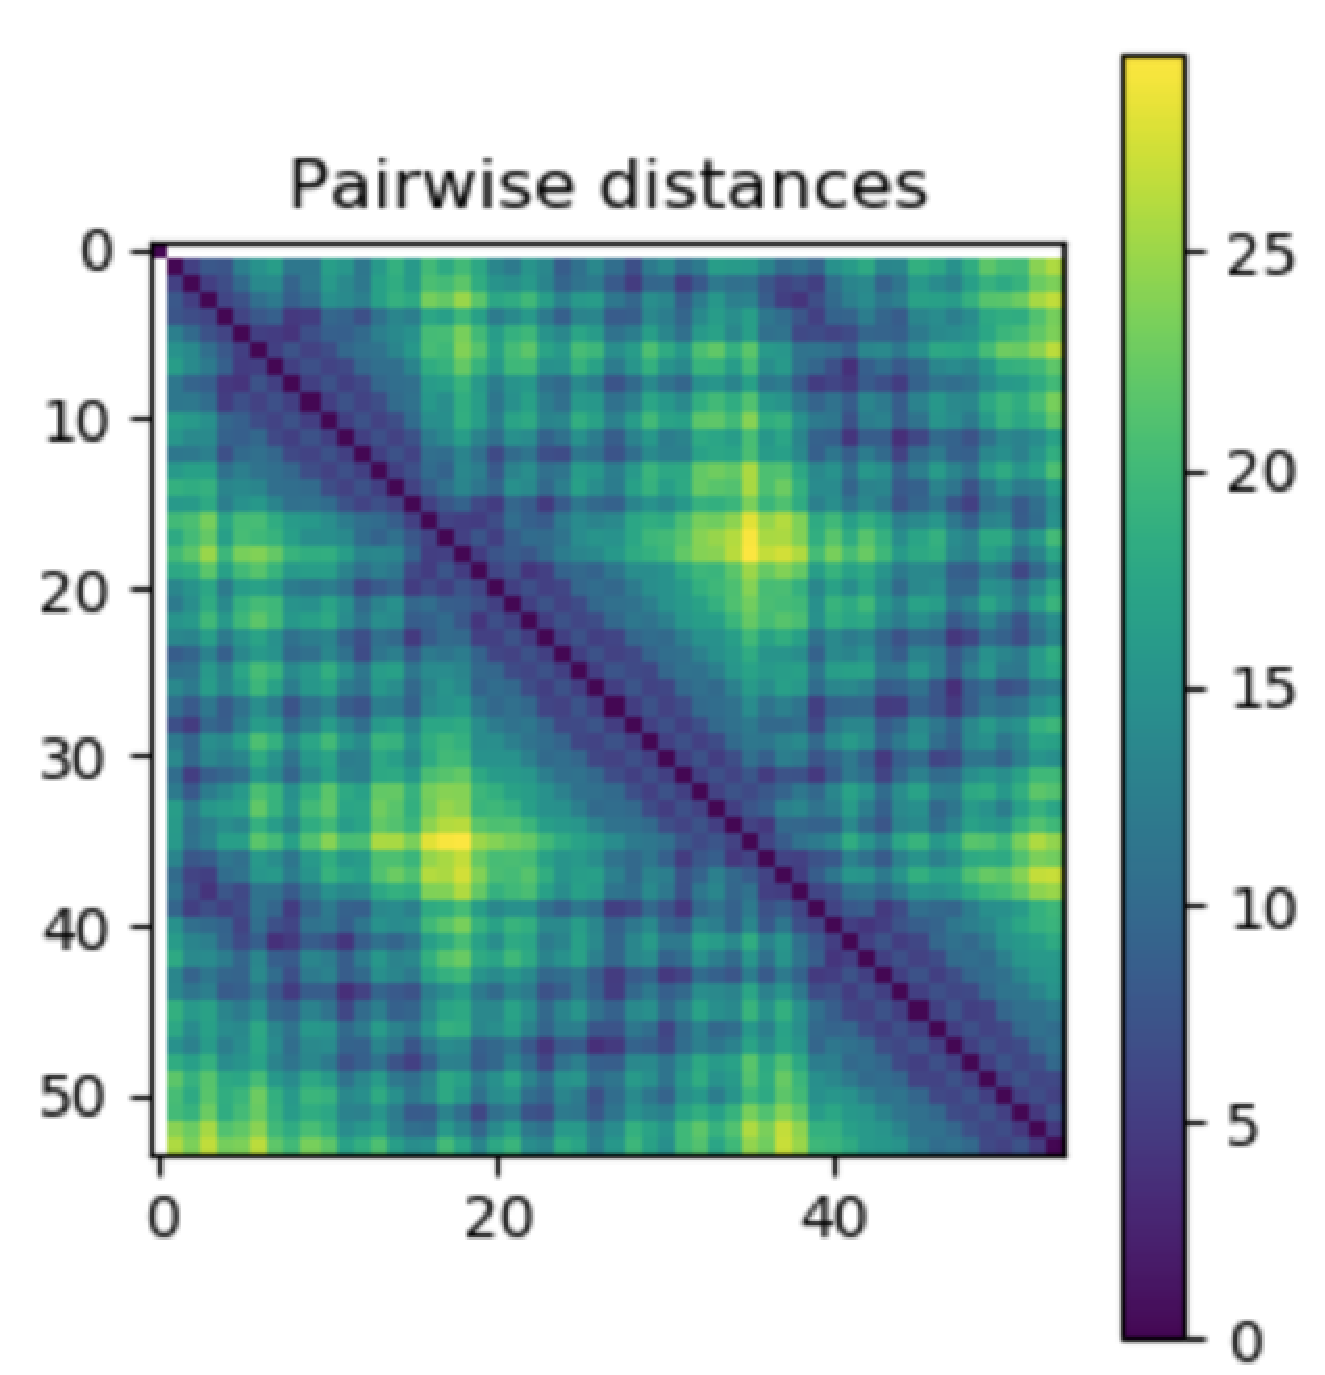
\includegraphics[width=\textwidth]{fig2.pdf}
					\caption{Попарные расстояния между элементами белка}
				\end{minipage}
			\end{figure}

			
			\subsection{Архитектуры сетей}
				\begin{enumerate}
					\item Deep Graph Convolutional Neural Network (DGCNN)\cite{Zhang2018AnED}
					\item 
					\item 
				\end{enumerate}
	
	\section{Результаты}
	
	
	

	\bibliographystyle{plain}
	\nocite{*}
	\bibliography{Severilov2019NIR}
	
\end{document}
